\chap{Fenómenos críticos del frente de infección}{resultados_criticos}
\graphicspath{{figs/cap5}}
\vspace*{-.3cm}
En este capítulo resolvemos numéricamente el modelo SIR espacial heterogéneo propuesto en el capítulo \ref{cap:SIR}. Es decir, el sistema
\begin{align}
    \partial_t S &=-\beta_{\vb r} SI + D_{S} \laplacian{S},\label{Seqdif}\\[.3cm]
    \partial_t I &=\beta_{\vb r} SI - \gamma I + D_{I} \laplacian{I},\label{Ieqdif}
\end{align}
con $(x,y) \in [0,L_x]\times[0,L_y]$ y condiciones iniciales
\begin{align*}
    I(x,y,0) &= 
    \begin{cases}
    I_0 & \text{si} \; (x,y) \in \Omega_0 \\
    0 & \text{si} \; (x,y) \notin \Omega_0  
    \end{cases}
    & ;&&
    S(x,y,0) &=
    \begin{cases}
    1-I_0 & \text{si} \; (x,y) \in \Omega_0 \\
    S_0 & \text{si} \; (x,y) \notin \Omega_0.
    \end{cases}
\end{align*}
donde $\Omega_0 = (0,\delta x) \times [0,Ly]$, es decir, la condición inicial consiste en un frente de infección plano. En cuanto a las condiciones de contorno tomamos condiciones periódicas en la dirección $y$ y condiciones de Dirichlet en la dirección $x$ dadas por
\begin{align*}
    I(0,y,t)=I(L_x,y,t)=S(0,y,t)=S(L_x,y,t)=0.
\end{align*}

Todas las simulaciones realizadas en este capítulo se realizaron sobre sistemas relativamente chicos de $1024\times 1024$\footnote{Comparados con los del capítulo \ref{cap:rugosidad}.}. Se decidió utilizar este tamaño de sistema dado que en este capítulo nos centramos en estudiar características macroscópicas del frente, las cuales presentan pequeñas fluctuaciones para diferentes realizaciones y transitorios cortos, de modo que un sistema de este tamaño resultó suficiente. Para referencia es importante decir que en este capítulo utilizamos un paso temporal de $0.05$ para integrar las ecuaciones, $Lx=Ly=1024$, $\delta x=1$ y $S_0=I_0=1$. Los demás parámetros del modelo se especificarán según corresponda.

En particular, vamos a estar observando la velocidad $c$, la amplitud máxima $I_{max}$ y la nocividad $S_1$ (a definir) del frente de infección en función del parámetro de desorden $p$ y la tasa de transmisión media espacial $\langle\beta_{\vb r}\rangle_{\vb r}=\beta_m$ para las distintas heterogeneidades. Veremos cómo cada uno de estos observables muestra un comportamiento crítico cerca del umbral de propagación y determinaremos los exponentes críticos asociados. En el camino discutiremos las diferencias de los resultados entre las heterogeneidades y las posibles interpretaciones en términos epidemiológicos. 

\vspace*{-.7cm}
\sect{Medio homogéneo (H)}{H}

Por completitud comenzamos mostrando los resultados numéricos obtenidos para el problema homogéneo, donde podemos corroborar con lo desarrollado analíticamente
en el capítulo \ref{cap:SIR}.

En la figura \ref{fig:h_case}a se muestra la evolución del frente de infección para el caso homogéneo, donde se utilizó $\beta=1$,$\gamma=0.2$, $D_S=0$ y $D_I=1$.
Nótese que $\beta > \beta_c = \frac{\gamma}{S_0} = 0.2$ de modo que la tasa de transmisión es mayor que la tasa de transmisión crítica y por lo tanto se observa una solución en forma de onda. Se muestra también (fig \ref{fig:h_case}a) el campo de desplazamiento del frente $u(y,t)$ (ecuación \ref{campo}), el cual es completamente plano, como es de esperar con una tasa de transmisión homogénea. Si se mira con detenimiento (fig. \ref{fig:h_case}b), puede observarse que el perfil del frente es asimétrico, es decir, se comporta de manera distinta en la parte frontal que en la parte posterior, tal como habíamos anticipado analíticamente en el capítulo \ref{cap:SIR}. Los perfiles asintóticos, frontal y posterior, coinciden con los obtenidos de las ecuaciones \ref{larika2} y \ref{larika} respectivamente.

\begin{figure}[!h]
    \centering
    \begin{subfigure}{1\textwidth}
      \centering
      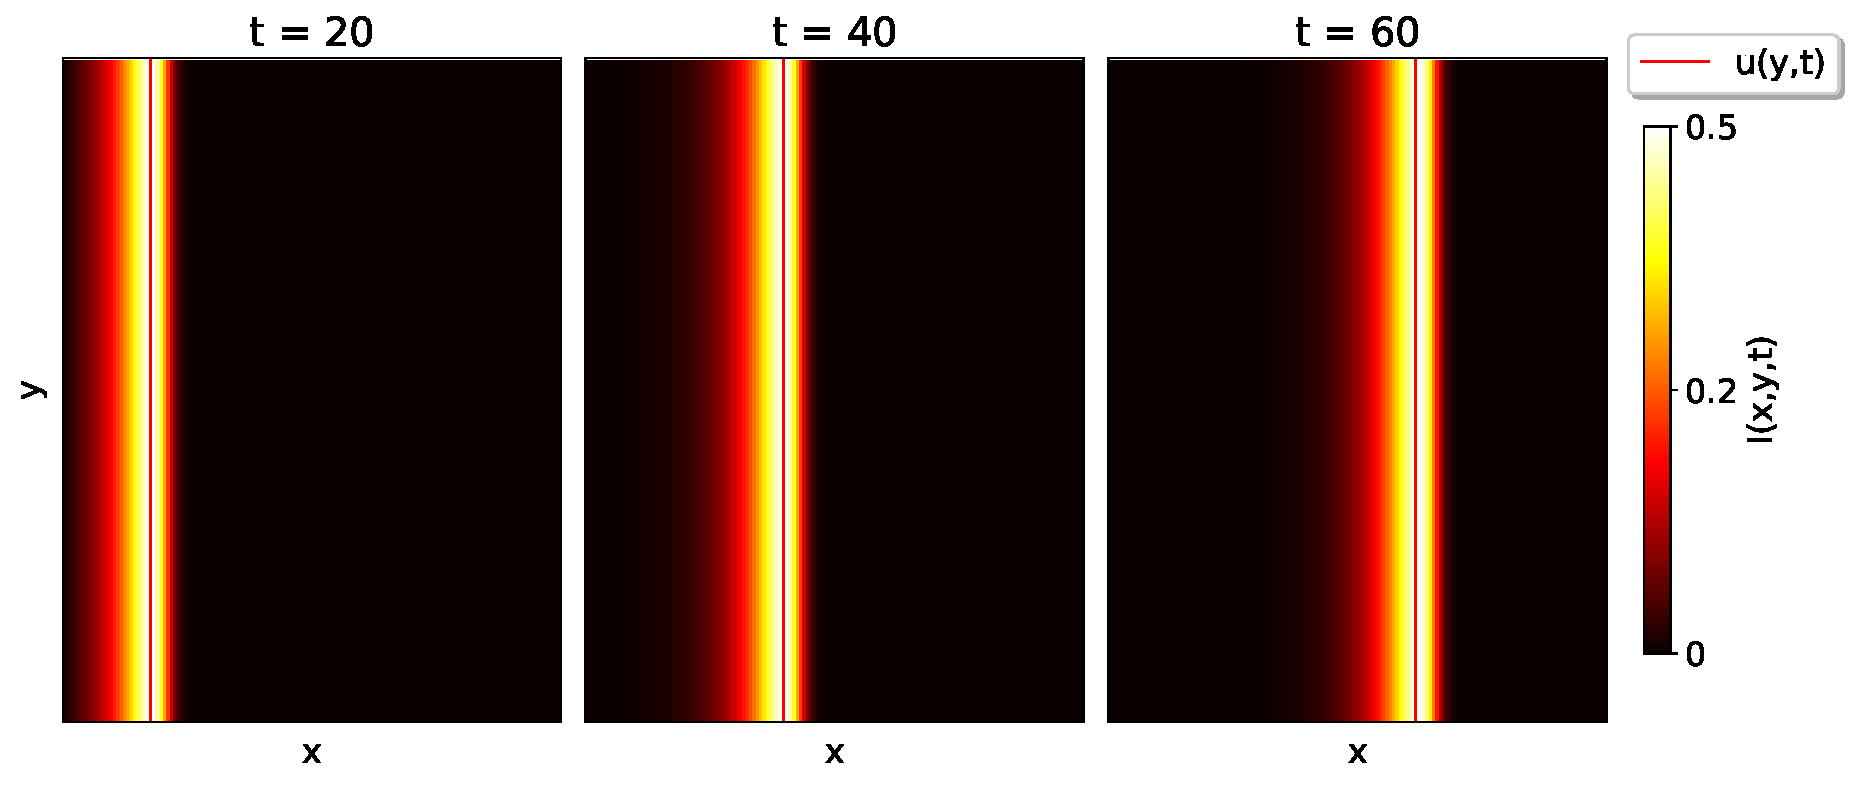
\includegraphics[width=.87\textwidth]{h_case.pdf}
      \caption{}
    \end{subfigure}
    \begin{subfigure}{1\textwidth}
      \centering
      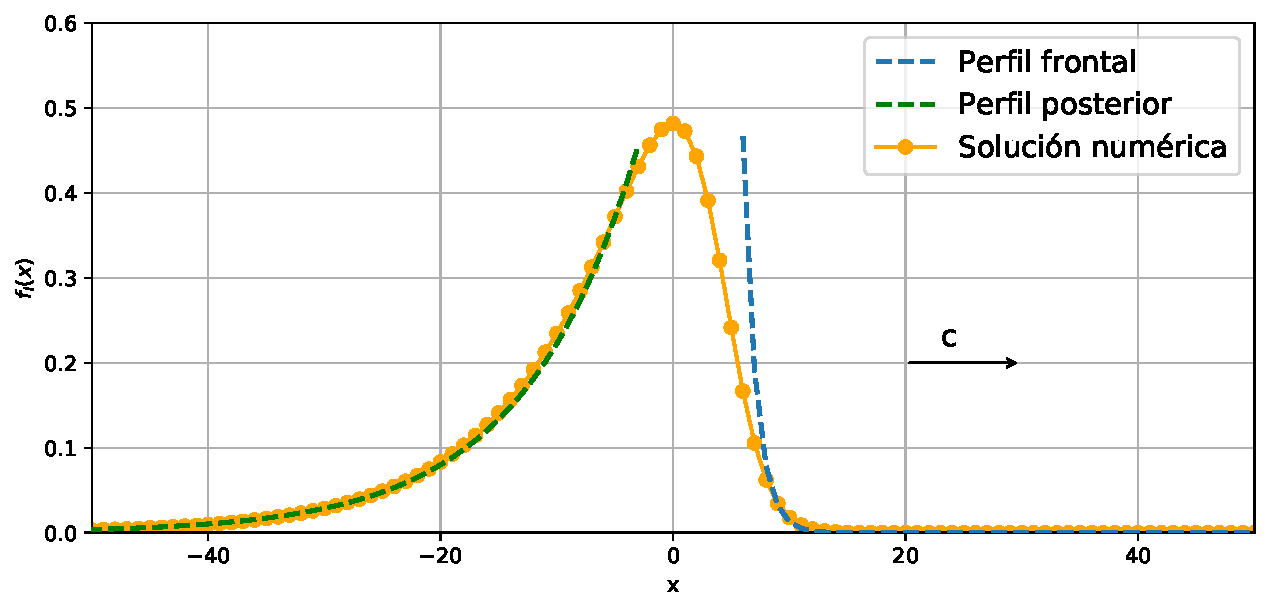
\includegraphics[width=.87\textwidth]{f_I(x)_hom.pdf}
      \caption{}
    \end{subfigure}
    \begin{subfigure}{1\textwidth}
        \centering
        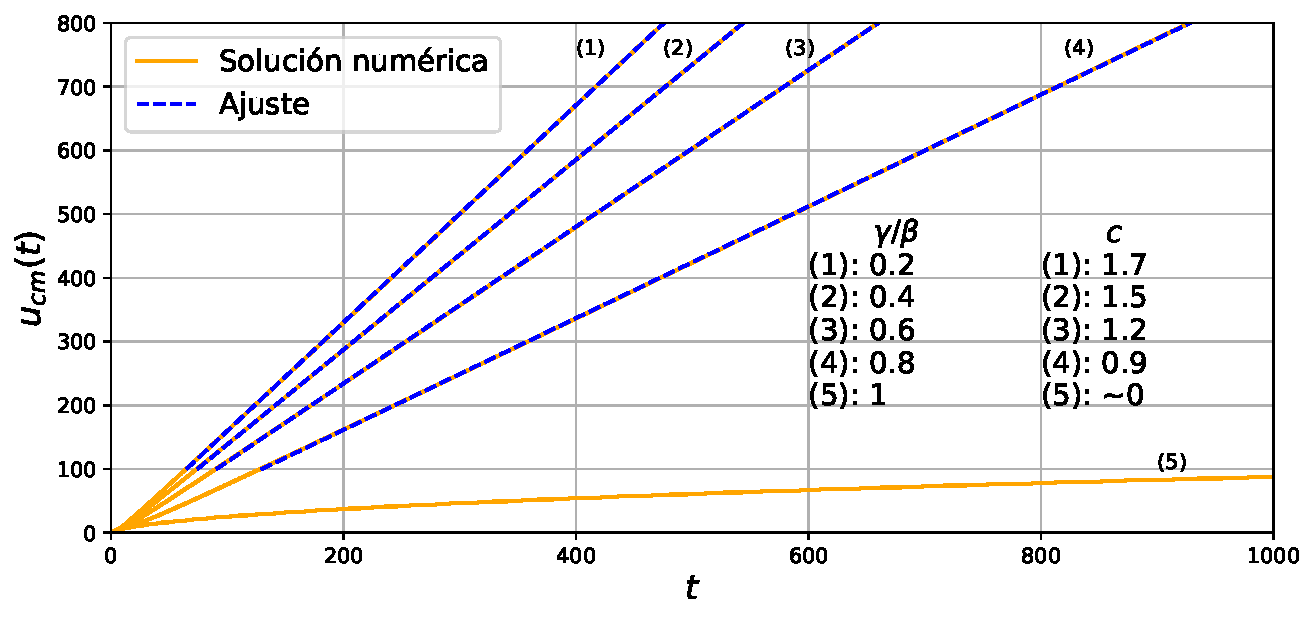
\includegraphics[width=.87\textwidth]{u_cm(t).pdf}
        \caption{}
    \end{subfigure}
    \caption[Representación del campo de infectados y evolución del centro de masa en medio H.]{\textbf{(a)} Mapa de color de la evolución del frente de infección sobre un medio homogéneo con parámetros $\beta=1$, $\gamma=0.2$, $D_S=0$ y $D_I=1$.
    \textbf{(b)} Perfil longitudinal del frente de infección, se muestran también los perfiles asintóticos frontal y posterior 
    del frente de onda calculados en la sección \ref{sec:modeloRDHo}. \textbf{(c)} Posición del centro de masa del frente de infección en función del tiempo para distintos valores de $\gamma/\beta$ junto con los correspondientes ajustes lineales. Se muestra también la velocidad $c$ obtenida para cada caso.}
    \label{fig:h_case}
\end{figure}

En la figura \ref{fig:h_case}c se muestra la posición del centro de masa del frente de infección $u_{cm}(t)$ (ecuación \ref{centromasa}) en función del tiempo para distintos valores de $\gamma/\beta$. Puede observarse 
que para el caso $\gamma/\beta=1$ el sistema cambia de comportamiento y no es posible identificar un frente de onda propagándose a velocidad constante y la amplitud del mismo se va a cero, en acuerdo con la condición de umbral $\gamma/\beta<S_0=1$. Por otro lado, se calculó la velocidad $c$ (ecuación \ref{velocidad}) para cada una de estas curvas descartando un período transitorio. De ello vemos que la velocidad del frente, estimada analíticamente $c_0 = 2\sqrt{D_I(\beta S_0-\gamma)}$, concuerda 
con las velocidades obtenidas numéricamente con un error relativo, en promedio, de $4.5\%$. 

En la mayoría de los casos $c_0$ resulta sobreestimar levemente el valor de $c$, sin embargo, $c_0$ originalmente era una cota mínima para la velocidad, ¿cómo puede ser? Esto puede explicarse recordando que el valor de $c_0$ se obtuvo en una aproximación lineal donde se supone que hay más susceptibles de los que realmente hay, por ello es de esperar que la cota mínima estimada $c_0$ sea sutilmente mayor que la real. En cualquier caso, se observa que el frente prefiere la velocidad mínima posible, esto es un fenómeno común en este tipo de sistemas \cite{Murray2002}.


\sect{Medios heterogéneos}{HET}

\ssect{DA vs H}{DA}

Vamos a comenzar estudiando el efecto que tiene la heterogeneidad DA en la solución del sistema. Para ello tendremos de referencia todo lo que sabemos del sistema sobre un medio H, tanto resultados analíticos como numéricos. La comparación entre DA y H nos permitirá entender mejor los efectos de la heterogeneidad.

Observando la figura \ref{fig:da}, que muestra el frente de infección propagándose sobre un medio DA con $p=0.3$, encontramos diferencias notables a simple vista con el frente sobre H (fig. \ref{fig:h_case}a). En principio, lo más notable es que el frente deja de ser plano y se vuelve rugoso. Esto es de esperar, ya que el frente ahora se encuentra con una fracción $p$ de lugares en donde no pueden darse contagios dado que la tasa de transmisión se anula, dando lugar a un avance tortuoso sobre el espacio, y fluctuante en el tiempo.

\begin{figure}[b]
    \centering
    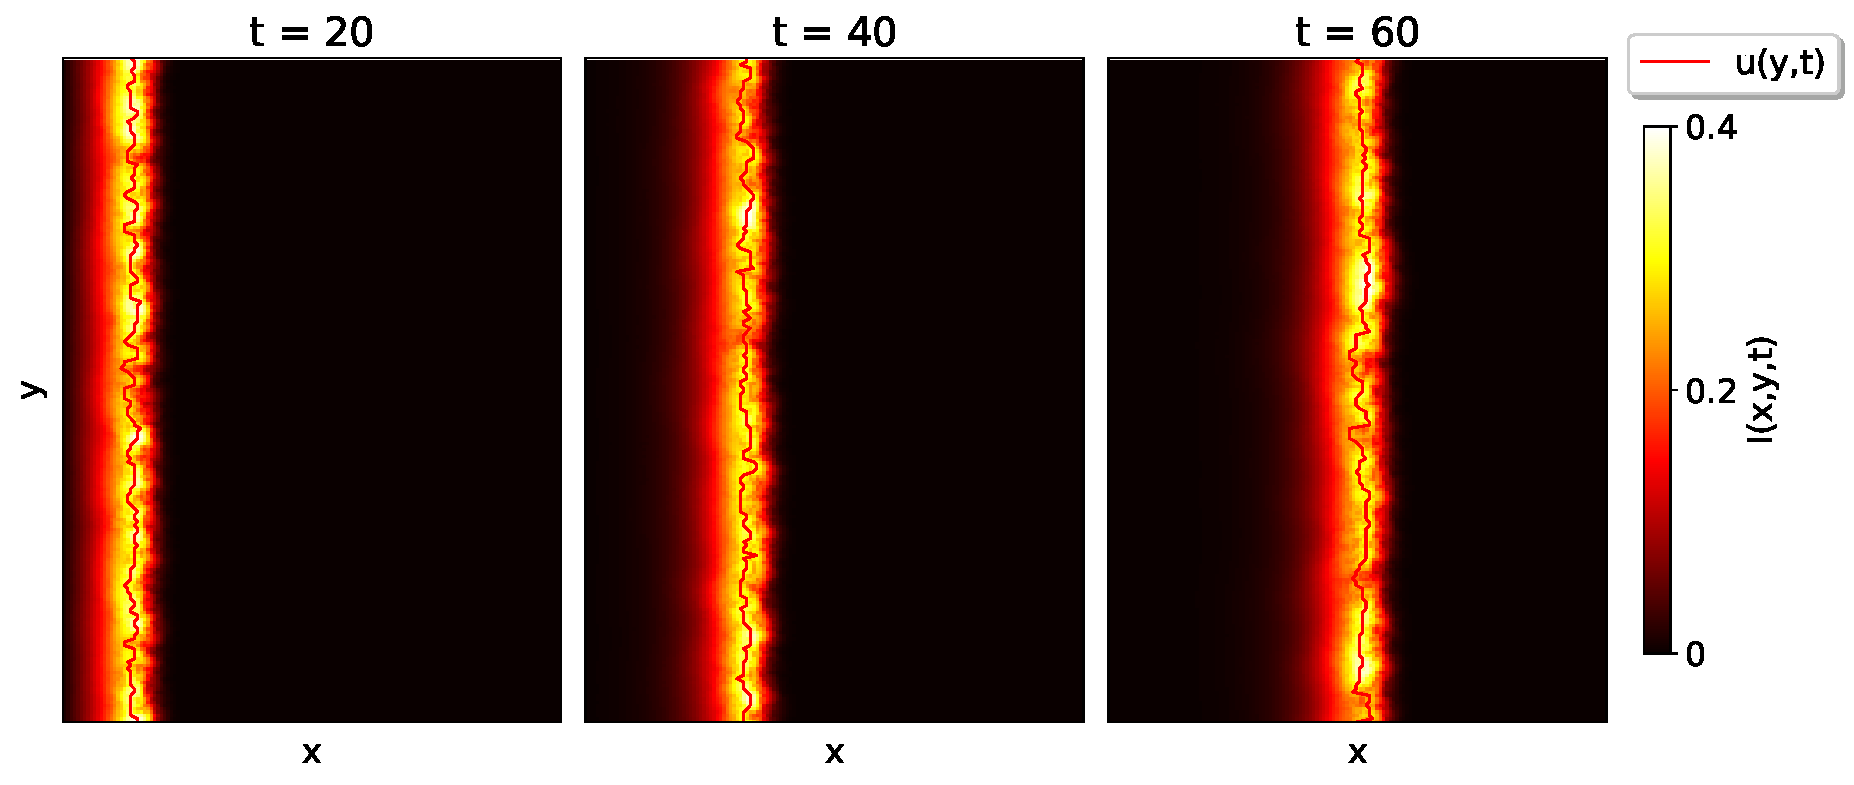
\includegraphics[width=\imsizeL]{da_case.pdf}
    \caption[Representación del campo de infectados y evolución del centro de masa en medio DA.]{Evolución del frente de infección sobre un medio heterogéneo DA con $p=0.3$, $\gamma=0.2$, $\beta=1$, $D_S = 0$ y $D_{I}=1$.}
    \label{fig:da}
\end{figure}

Sin embargo, podemos hacer algunas preguntas más difíciles, por ejemplo, ¿cuál es el umbral de propagación para el caso DA?, ¿cuál es la velocidad del frente?,
¿dada la misma tasa de transmisión espacial media, es más rápido el frente sobre el medio DA o sobre el medio H? 

\begin{equation}
    p\;,\;1 - \frac{\beta^H}{\beta ^{DA}}
\end{equation}

\subsubsection*{Velocidad y umbral de propagación}

\begin{figure}[!b]
    \centering
    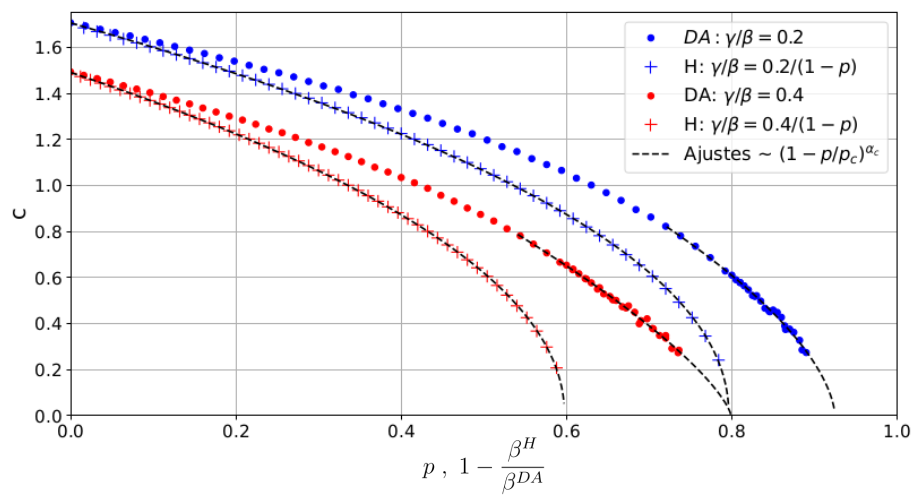
\includegraphics[width=\imsizeL]{cc.png}
    \caption[Velocidad del frente infección en función del parámetro de desorden $p$.]{Velocidad $c$ del frente de infección en función de $p$ para los medios H y DA con la misma tasa de transmisión media espacial usando $\gamma/\beta=0.2$ y $0.4$, $D_S=0$ y $D_{I}=1$. Se muestran los ajustes con la regla de potencia $c\propto(1-p/p_c)^{\alpha_c}$ sobre la región crítica.}
    \label{fig:velocidad_p}
\end{figure}

Uno podría intentar responder estas preguntas pensando en una aproximación de campo medio en la que usamos los resultados del caso H, pero reemplazamos $\beta$ por la tasa de transmisión media espacial $\langle\beta_{\textbf{r}}\rangle_{\textbf{r}} = \beta_m$ del medio DA. Asumiendo un sistema de tamaño infinito, entonces la tasa de transmisión media espacial es igual a la tasa de transmisión media sobre desorden, es decir,
\begin{equation}
    \beta_m = \overline{\beta_{\vb r}} = \beta(1-p).
\end{equation}
De esta manera, en lo que respecta al umbral, vimos que en el caso homogéneo la tasa de transmisión crítica a partir de la cual se sostiene un frente de onda es, $\beta_c=\frac{\gamma}{S_0}$. Reemplazando este $\beta_c$ por $\beta_m$ encontramos entonces un valor crítico \textit{naive} para el parámetro de desorden $p_c$ dado por,
\begin{equation}
    p_c = 1 - \frac{\gamma}{\beta S_0},
\end{equation}
que define el umbral de propagación. Haciendo algo similar, reemplazando $\beta_m$ por $\beta$ en la expresión para la velocidad del frente en el caso homogéneo $c_0$ (ecuación \ref{eq:c0}), encontramos lo que sería la velocidad del frente en función de $p$,
\begin{equation}
    c(p) = c_0\left(1-\frac{p}{p_c}\right)^{1/2}.
\end{equation}

Desafortunadamente, o quizás afortunadamente, estos resultados predicen incorrectamente los valores obtenidos de las simulaciones. En la figura \ref{fig:velocidad_p} se muestra la velocidad del frente,
\begin{equation}
    c = \langle c(t)\rangle_t = \langle \overline{\dot{u}_{cm}(t)}\rangle_t
\end{equation}
para distintos valores del parámetro de desorden $p$ sobre el medio DA, ignorando un transitorio. En la misma se observa efectivamente un fenómeno crítico donde la velocidad del frente se anula siguiendo una ley de potencia del tipo $c \propto (1-p/p_c)^{\alpha_c}$, sin embargo, tanto el exponente crítico $\alpha_c$ como el umbral de propagación $p_c$ no coinciden con los valores predichos por la aproximación de campo medio. En la tabla \ref{tab:param_criticos} se pueden observar los valores obtenidos ajustando la ley de potencias en los resultados para la velocidad.

Se observa que las curvas de velocidad sobre el medio H en función de $p =1 - \beta$ concuerdan con los resultados obtenidos analíticamente (tabla \ref{tab:param_criticos}), por ejemplo con $(\gamma=0.2,S_0=~1)$, resulta que $p_c = 0.8\pm 0.01$ que concuerda con $\beta_c = 1- p =  0.2$. De igual manera, los exponentes críticos obtenidos $\alpha_c\approx 0.5$ también coinciden con la expresión para la velocidad $c_0$ del caso homogéneo.



Por otro lado, calculamos la velocidad del frente sobre un medio H con la misma tasa de transmisión media espacial que la de un medio $DA$ con un dado $p$ (fig. \ref{fig:velocidad_p}), es decir, tomamos $\beta^H = \beta ^{DA}(1-p)$. \textbf{Resulta que el frente de infección es más veloz sobre el medio DA que sobre el medio H dada la misma tasa de transmisión media espacial.} Esto sugiere que la heterogeneidad introducida en el sistema da lugar a un efecto de aceleración del frente de infección. Esta aceleración no puede explicarse utilizando una tasa de transmisión efectiva igual a la tasa de transmisión media espacial del medio DA. Se trata de un fenómeno emergente no trivial. En términos epidemiológicos, si uno piensa en $p$ como la fracción de lugares donde la población está vacunada o en cuarentena, entonces una estrategia de vacunación o cuarentena con distribución espacial de tipo DA daría lugar a un frente de infección más veloz que una estrategia de vacunación o cuarentena espacialmente homogénea.

Más aún, no solo hay un efecto de aceleración, si no que el umbral de propagación se reduce a un valor de transmisión media espacial menor en el medio DA. Esto es, tal como se muestra en la figura \ref{fig:velocidad_p}, dados $(\gamma=0.2,S_0=1)$ la tasa de transmisión crítica en un medio H es $\beta_c =~ \gamma/S_0=~0.2$. Sin embargo, en un medio DA con estos parámetros obtenemos el valor crítico $p_c = 0.92\pm 0.04$, lo que se traduce en una tasa de transmisión media de $\beta_m = \beta (1-p) \approx 0.08$. Es decir, es más fácil propagar la infección en un medio DA que en un medio H dada la misma tasa de transmisión media espacial.

\textbf{Por lo tanto, la ``homogeneización'' \textit{naive} no es una buena aproximación: subestima el umbral y la velocidad de propagación.}

\begin{table}[!b]
    \centering
    \caption{Parámetros críticos $p_c$ y $\alpha_c$ de los medios H y DA con diferentes $\gamma/\beta$.}
    \label{tab:param_criticos}
    \begin{tabular}{@{}cccc@{}}
    \toprule
    Medio & $\gamma/\beta$ & $p_c$         & $\alpha_c$    \\ \midrule
    DA    & 0.2            & $0.92\pm0.04$ & $0.6\pm0.1$ \\
    H     & 0.2            & $0.80\pm0.01$ & $0.47\pm0.04$ \\
    DA    & 0.4            & $0.80\pm0.04$ & $0.7\pm0.1$ \\
    H     & 0.4            & $0.60\pm0.01$ & $0.48\pm0.04$ \\ \bottomrule
    \end{tabular}
\end{table}


Por lo visto hasta ahora uno pensaría, al menos en términos epidemiológicos, que es preferible tener una tasa de transmisión con una distribución homogénea antes que una de tipo DA, ya que así habría una propagación más lenta. Sin embargo, antes de asegurar esto debiéramos tener en cuenta otras características epidemiológicas relevantes. Una de ellas es la amplitud del frente, una amplitud grande del frente implicaría muchos individuos infectados al mismo tiempo, lo cual podría demandar una cantidad de recursos e infraestructura de salud simultáneamente inaccesible. Esto podría producir fácilmente el colapso de los servicios de salud dando lugar a muchas tragedias. 
Entonces, ¿cómo es la amplitud del frente sobre el medio DA en comparación con H?


\subsubsection*{Amplitud del frente}

De manera similar a lo que hicimos con la velocidad del frente, calculamos la amplitud del mismo sobre los medios H y DA. Más precisamnete, tomamos un valor para cada simulación promediando temporalmente y descartando un transitorio, es decir,

\begin{equation}
    I_{max} = \langle I_{max}(t) \rangle_{t}.
\end{equation}

Los resultados obtenidos se muestran en la figura \ref{fig:amplitud_p}. En primer lugar observamos que la amplitud del frente se anula en los mismos valores de $p_c$ en los que se anula la velocidad. Esto es razonable dado que al detenerse, el frente de infección no puede encontrar nuevos susceptibles, de modo que los infectados terminan recuperándose en un período $\frac{1}{\gamma}$ y la amplitud del frente se anula. 

\begin{figure}[!b]
    \centering
    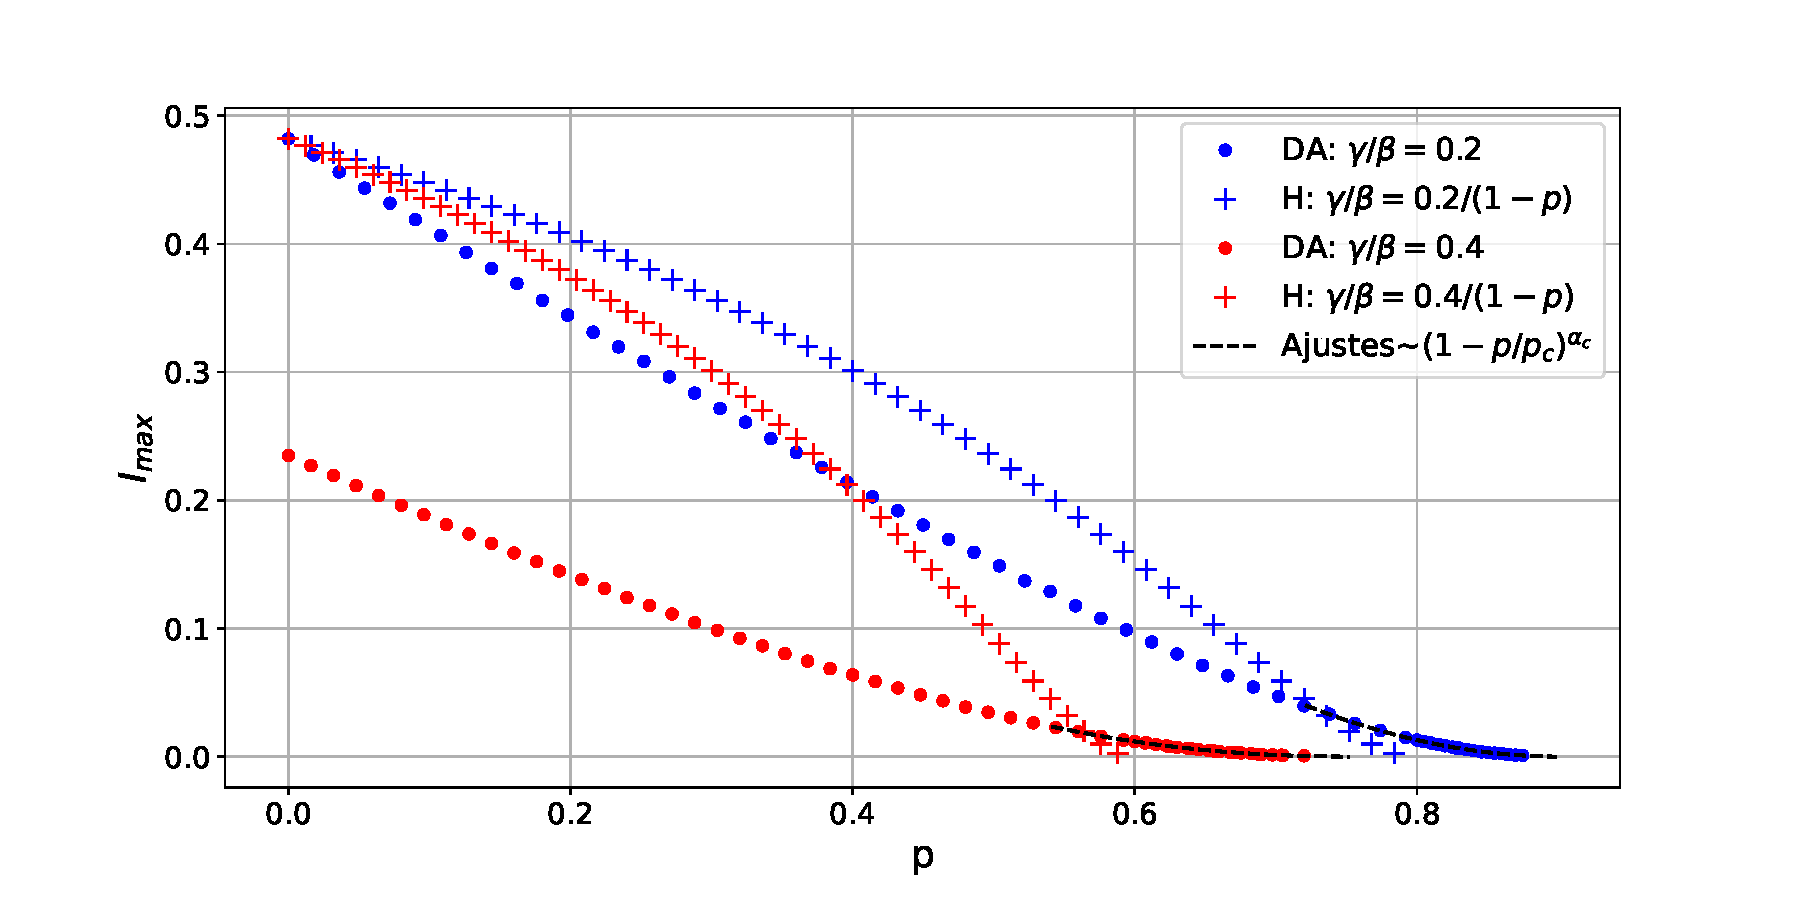
\includegraphics[width=\imsizeL]{amplitud_p.pdf}
    \caption[Amplitud máxima del frente de infección en función del parámetro de desorden $p$]{Amplitud media $I_{max}$ del frente de propagación en función de $p$ con $\gamma/\beta=0.2$ y $0.4$ y $D_{I}=1$. Se muestran los 
    ajustes con la regla de potencia $I_{max}\propto(1-p/p_c)^{\alpha_I}$ sobre la región crítica.}
    \label{fig:amplitud_p}
 \end{figure}

Por otro lado, más interesante, vemos que dados los mismos parámetros y la misma tasa de transmisión media espacial, \textbf{la amplitud máxima del frente es mayor sobre el medio H que sobre el medio DA en tanto $p<p_c^H$, donde $p_c^H$ es el umbral del medio H.} De modo que, al contrario de lo que sucede con la velocidad, la heterogeneidad introducida en el sistema da lugar a un efecto de disminución de la amplitud del frente. En este sentido entonces es preferible una distribución DA antes que una H. 

Es posible relacionar los resultados de la velocidad y la amplitud conceptualmente de la siguiente manera: en general, si un frente de infección es más rápido entonces pasa menos tiempo localizado en un lugar, consecuentemente se contagia menos gente en ese lugar y por lo tanto la amplitud es menor, si el frente es lento se da el efecto contrario.

Observamos también que la amplitud máxima media sigue una ley de potencias $I_{max} \propto (1-p/p_c)^{\alpha_I}$ con exponente crítico $\alpha_I$. En la tabla \ref{tab:param_criticos_I} mostramos los valores de $p_c$ y $\alpha_I$ obtenidos con este ajuste. Se ve que en ambos casos el exponente crítico es aproximadamente igual a 2.


 \begin{table}[t]
    \centering
    \caption{Parámetros críticos $p_c$ y $\alpha_I$ del medio DA con diferentes $\gamma/\beta$.}
    \label{tab:param_criticos_I}
    \begin{tabular}{@{}cccc@{}}
    \toprule
    Medio & $\gamma/\beta$ & $p_c$         & $\alpha_I$    \\ \midrule
    DA    & 0.2            & $0.90\pm 0.04$ & $1.93 \pm 0.05$ \\
    DA    & 0.4            & $0.75\pm 0.04$ & $2.12 \pm 0.05$ \\ \bottomrule
    \end{tabular}
\end{table}

 En resumen, observamos que para decidir en términos epidemiológicos qué distribución $\beta_{\vb r}$ es más conveniente, es necesario primero decidir si es preferible un frente rápido con menor amplitud o uno rápido con mayor amplitud. Para ello quizás sea conveniente definir otra magnitud. Quizás lo interesante sea pensar que las epidemias se dan en espacios finitos, de modo que lo importante en definitiva sería saber qué daño causará realmente el frente de infección en determinado espacio. Para ello vamos a introducir lo que llamamos \textit{nocividad} $S_1$ del frente de infección, la cual se definirá más adelante a la vez que mostramos resultados sobre las demás heterogeneidades. 
 
Los resultados obtenidos hasta aquí de la comparación entre el medio H y el DA pueden describirse cualitativamente de la siguiente manera: 
 \begin{itemize}
     \item Si el valor medio espacial de la tasa de transmisión $\beta_m$ es el mismo, la velocidad del frente de infección es \textit{mayor} sobre el medio 
     DA que sobre el H.
     \item Si el valor medio espacial de la tasa de transmisión $\beta_m$ es el mismo, la amplitud máxima media del frente de infección $I_{max}$ es 
     \textit{mayor} sobre el medio H que sobre el DA en tanto $p<p_c^H$, con $p_c^{H}$ el umbral del medio H.
     \item El valor de umbral de la tasa de transmisión media $\beta_m$ para el cual se extingue el frente de infección es \textit{menor} sobre el medio DA que sobre el H.
     \item Los exponentes críticos de la velocidad $\alpha_c$ para el medio homogéneo \textit{coinciden} con el estimado por $c_0$ en la aproximación analítica de la solución de onda. $(\alpha_c = \frac{1}{2})$
     \item Los exponentes críticos de la velocidad $\alpha_c$ para el medio DA son aparentemente \textit{mayores} que para el medio H. Sin embargo, más precisión es necesaria para decidir si $\alpha_c$ es universal o no. ($\alpha_c\approx0.5$)
 \end{itemize}

 
\ssect{Medios correlacionados}{corr}

En esta sección sumamos a los resultados los efectos de las heterogeneidades con correlación, es decir, la heterogeneidad <<suavizada>> (S) y la <<dicotómica-correlacionada>> (DC) únicamente con $n = 1$, un paso del algoritmo que genera S y DC discutido en el capítulo \ref{cap:SIR}.


A continuación mostramos los resultados de velocidad y amplitud del frente de infección sobre todos los medios propuestos. La diferencia es que ahora estaremos viendo los resultados directamente en función de la tasa de transmisión media $\beta_m$ en lugar de $p$.


\subsubsection*{Velocidad y amplitud del frente}

En la figura \ref{fig:c_all} se muestra la velocidad en función de la tasa de transmisión media espacial $\beta_m$ para todos los medios, H, DA, S y DC. En primer lugar observamos que la curva asociada al medio S cae entre las curvas del medio H y el medio DA. Esto es razonable dado que el medio S se genera del medio DA y tiende a un homogéneo cuanto más los suavizamos.

Por otro lado, la curva de velocidad asociada al medio DC muestra la mayor velocidad del frente infección de todos los medios. Este resultado es muy interesante, es decir, \textbf{un ligero cambio en la estructura del medio, sin modificar la tasa de transmisión media, produce un cambio notable en la velocidad del frente}. Fundamentalmente, comparando el resultado de DC con el de DA, a pesar de que ambos medios tengan un carácter dicotómico, la correlación espacial
introducida en DC genera un cambio apreciable sobre la velocidad.

\begin{figure}[!b]
    \centering
    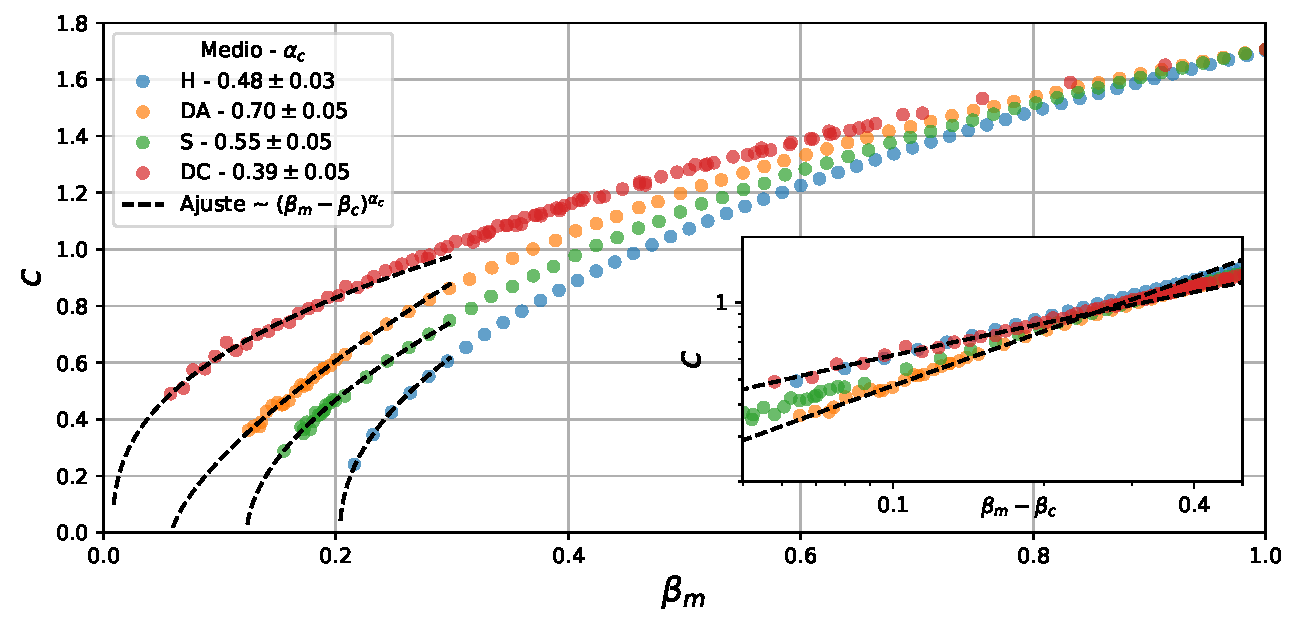
\includegraphics[width=\imsizeL]{c_all.pdf}
    \caption[Velocidad del frente de infección en función de $\beta_m$ para los medios H, S, DA y DC]{Velocidad del frente de infección en función del valor medio de la tasa de transmisión $\beta_m$ sobre los medios S, DC, DA y 
    H. Se muestran los ajustes con la regla de potencia $c\propto(\beta_m-\beta_c)^{\alpha_c}$ sobre la región crítica.}
    \label{fig:c_all}
\end{figure}

Para entender mejor qué es lo que produce este cambio de velocidad entre DA y DC es interesante observar con mayor detenimiento la estructura de estos medios. En las 
figuras \ref{beta_al_zoom} y \ref{beta_dic_zoom} se muestra la distribución de la tasa de transmisión $\beta_{\vb r}$ sobre el espacio de los medios DA y DC respectivamente, donde ambos tienen la misma tasa de transmisión media espacial. Observando la distribución espacial de cada uno de ellos 
a gran escala, sobre el espacio de $1024\times1024$, no es sencillo señalar ninguna diferencia. Sin embargo, al observar la distribución sobre una región acotada de 
$100\times100$ se puede ver que son estructuralmente distintos en esta escala. La distribución de DC con $n=1$ alcanza a formar un patrón  
distinguible, se forman regiones agrupadas con tasa de transmisión no nula $\beta$, mientras que en DA, por supuesto, se observa el carácter aleatorio. Es decir, la velocidad de propagación es mayor si la distribución de la tasa de transmisión forma estructuras como las que se ven en la figura 
\ref{beta_dic_zoom} en lugar de estar distribuida aleatoriamente, por más que la tasa de transmisión media sea la misma.

\begin{figure}[t]
    \centering
    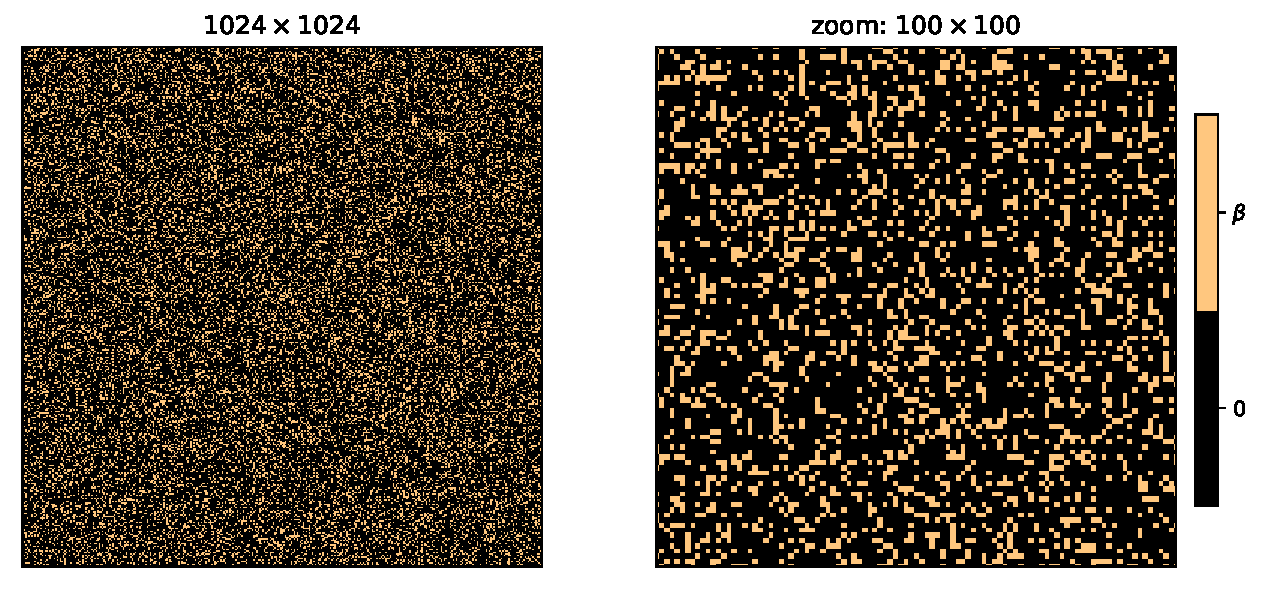
\includegraphics[width=\imsize]{beta_al_zoom.pdf}
    \caption[Medio DA en diferentes escalas]{Distribución de la tasa de transmisión $\beta_{\vb r}$ del medio DA. A izquierda se muestra la distribución sobre 
    todo el espacio de $1024\times1024$ y a la derecha un acercamiento a una región de $100\times100$.}
    \label{beta_al_zoom}
\end{figure}
\begin{figure}[t]
    \centering
    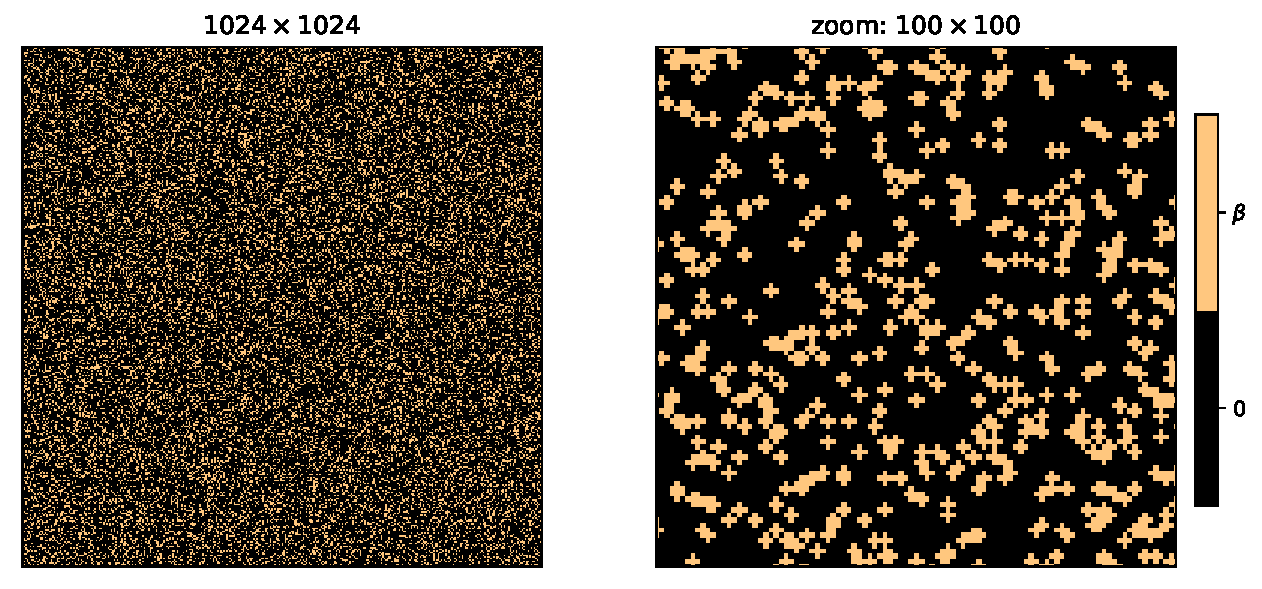
\includegraphics[width=\imsize]{beta_dic_zoom.pdf}
    \caption[Medio DC en diferentes escalas]{Distribución de la tasa de transmisión $\beta_{\vb r}$ del medio DC. A izquierda se muestra la distribución sobre 
    todo el espacio de $1024\times1024$ y a la derecha un acercamiento a una región de $100\times100$.}
    \label{beta_dic_zoom}
\end{figure}

Se realizaron ajustes con la ley de potencia $c\propto(\beta_m-\beta_c)^{\alpha_c}$ para las curvas de velocidad en la cercanía del umbral de propagación para los medios DC, DA, S y H. De ello se determinó la tasa de transmisión crítica $\beta_c$, que define el umbral de propagación, y el exponente crítico $\alpha_c$ para cada uno de ellos. En la tabla \ref{tab:pc} se muestran los resultados obtenidos.

\begin{table}[t]
    \centering
    \caption{Parámetros críticos $\beta_c$ y $\alpha_c$ de los medios DC, DA ,S y H.}
    \label{tab:pc}
    \begin{tabular}{@{}cccc@{}}
    \toprule
    Medio & $\beta_c$     & $\alpha_c$    \\ \midrule
    H     & $0.20\pm0.01$ & $0.48\pm0.05$ \\
    DA    & $0.06\pm0.02$ & $0.7\pm0.1$ \\
    DC    & $0.01\pm0.01$ & $0.4\pm0.1$ \\
    S     & $0.12\pm0.02$ & $0.6\pm0.1$ \\ \bottomrule
    \end{tabular}
\end{table}

De estos resultados también queda claro otro fenómeno notable al que da lugar la estructura del medio DC, y es que sobre este la tasa 
de transmisión crítica es \textit{menor} comparada con las demás. Es decir, basta con una tasa de transmisión extremadamente chica, comparada con los demás medios,
para que tenga lugar un frente de infección.

Por otro lado, en la figura \ref{fig:I_all} se muestran los resultados de la amplitud del frente en función de la tasa de transmisión media para los distintos medios. Observamos que el medio homogéneo es el que sostiene la mayor amplitud del frente de infección en tanto $\beta_m > 0.35$. Vemos aquí nuevamente que la curva de S queda entre las dadas por H y DA. Por otro lado, el medio DC, en consistencia con lo observado para la velocidad, otorga la mayor amplitud del frente para valores bajos de la tasa de transmisión media $\beta_m<0.35$. Es decir, el medio DC favorece nuevamente, en este aspecto y sobre este régimen, a la propagación del frente.

Sin embargo, nuevamente, no queda claro si es preferible un medio sobre otro, dado que observamos sistemáticamente que cuando la velocidad del frente es mayor la amplitud del mismo es menor en comparación con los frentes de menor velocidad. Para tratar de obtener un criterio más sobre el que juzgar introducimos la \textit{nocividad} de los frentes y vemos cómo es en cada medio.

\begin{figure}[h]
    \centering
    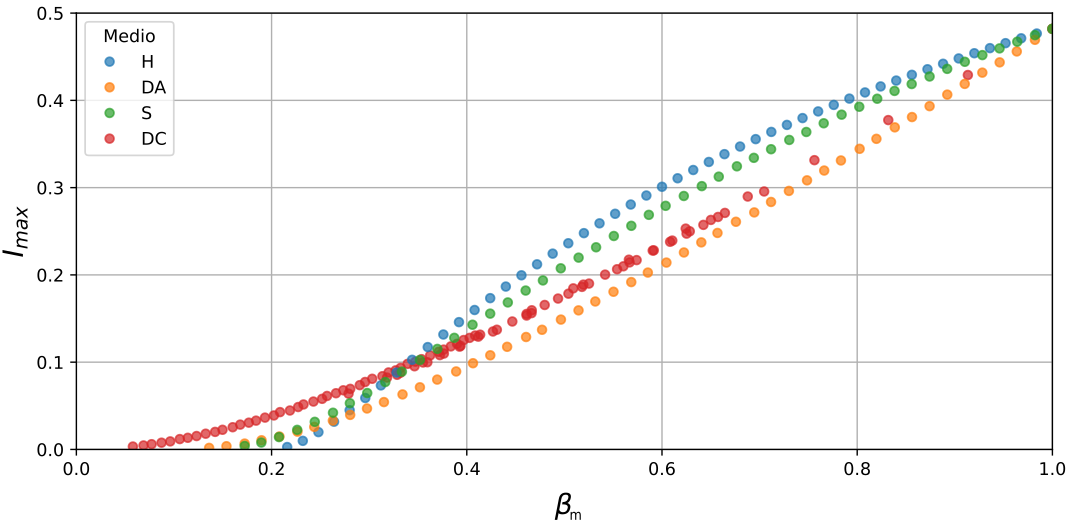
\includegraphics[width=\imsizeL]{I_max.png}
    \caption[Amplitud máxima en función de $\beta_m$ para los medios H, DA, S y DC]{Amplitud media del frente de infección/incendio $I_{max}$ en función de la tasa de transmisión media $\overline{\beta_{\vb r}}$ para los medios S, DA, 
    DC y H.}
    \label{fig:I_all}
\end{figure}


\newpage
\subsubsection*{Nocividad}

Un aspecto de gran importancia en lo que respecta a problemáticas tanto epidemiológicas como de incendios es la posibilidad de cuantificar los daños que
deja un brote de enfermedad infecciosa o un incendio. En particular, estaremos interesados en estimar el daño que queda tras el paso del frente de infección/incendio sobre una dada región. Para ello utilizaremos como cuantificador de daños la fracción de susceptibles remanentes $S_1$ que queda tras el paso del frente. Entendiendo que mientras menor sea esta fracción, mayor será el daño ocasionado por el frente.

Para ser más precisos al respecto, tomaremos 
\begin{equation}
    S_1=\langle S(x,y,T)\rangle_{x,y} \label{S1}  
\end{equation}
con $0.2L_x<x<u_{cm}(T)-0.2L_x$, siendo $T$ el tiempo que dure la simulación correspondiente\footnote{Notar que T varía en cada realización, fundamentalmente dado que la velocidad de los frentes en los distintos medios cambia. De modo que esta definición pone el foco en el daño que se hace en una dada región sin importar el tiempo que le lleve al frente recorrerla.}. Definido de esta manera $S_1$, quitamos los efectos del transitorio que se da en la primera región de evolución del sistema y posibles efectos de tamaño finito por estar cerca de los bordes de la región de simulación. Además imponemos que $x$ se encuentre relativamente lejos del centro de masa del frente para no contar los susceptibles en la región del frente mismo.

Utilizando este criterio para todas las simulaciones, podremos comparar 
la nocividad de cada frente al modificar los parámetros que interesen. En particular, veremos cómo cambia esta magnitud $S_1$ con la tasa de transmisión media espacial
$\beta_m$.

En la figura \ref{fig:S_1} se muestran los resultados obtenidos de $S_1$ en función de $\beta_m$ sobre los medios H, S, DA y DC. Se puede 
observar que el frente de propagación más nocivo se da sobre el medio homogéneo, ya que da lugar a la menor fracción de susceptibles $S_1$ tras el paso del frente. Sin 
embargo, tal como ya hemos apreciado antes (Tabla \ref{tab:pc}), la tasa de transmisión crítica es mayor que en los demás casos $\beta_c\approx0.2$.

\begin{figure}[!t]
    \centering
    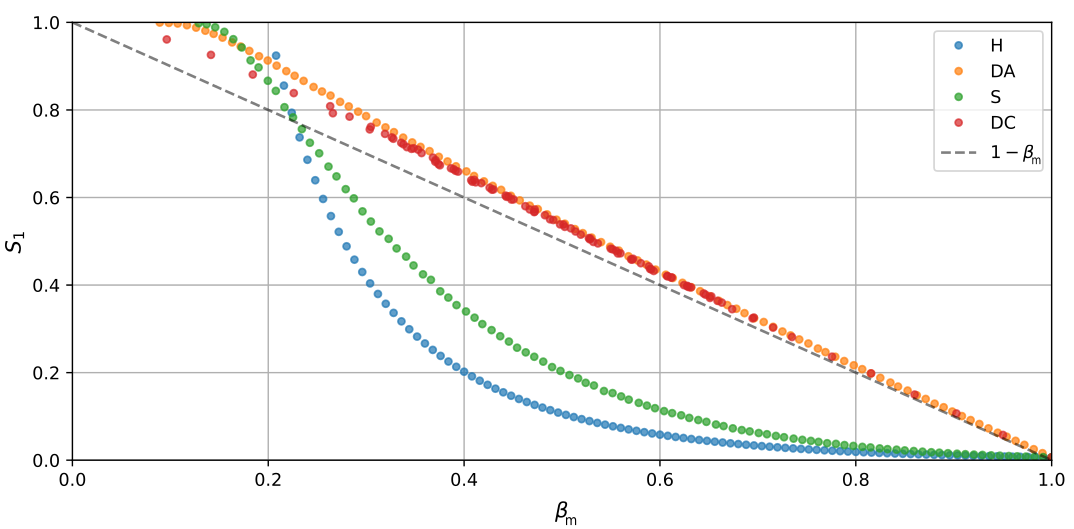
\includegraphics[width=\imsizeL]{S1_all.png}
    \caption[Susceptibles remanentes $S_1$ en función de $\beta_m$ para los medios H, S, DA y DC]{Susceptibles remanentes $S_1$ en función de la tasa de transmisión media $\beta_m$ para los medios H, S, DA y DC. Se muestra también la curva $1-\beta_m$ que aproxima $S_1$ sobre los medios dicotómicos.}
    \label{fig:S_1}
\end{figure}

El siguiente medio de nocividad elevada es S, mientras que los medios DC y DA presentan curvas similares de carácter lineal. Estos nuevos resultados dan una perspectiva 
nueva acerca de los medios. Por ejemplo, habíamos visto que la velocidad de propagación del frente es mayor sobre el medio DC que sobre los demás, lo cual es una 
característica indeseable en problemáticas tanto epidemiológicas como de incendios. Sin embargo, vemos ahora que a pesar de ello la nocividad del frente, tal como la
hemos caracterizado aquí, es menor sobre DC que sobre los demás medios, lo cual es deseable. A modo cualitativo es entendible que si el frente se desplaza a mayor 
velocidad tenga menos tiempo de ocasionar grandes daños. 

Respecto al carácter lineal que presentan las curvas de $S_1$ sobre los medios dicotómicos, podemos hacernos una idea de a qué se debe: los susceptibles en los lugares donde la tasa de transmisión es nula resultan completamente inaccesible al frente dado que solo hemos trabajo con el término difusivo de infectados en las ecuaciones del sistema (\ref{Seqdif} - \ref{Ieqdif}), ($D_S = 0,D_I=1$). Es decir, los infectados pueden ingresar a esas zonas, donde no pueden contagiar a nadie dado que la tasa de transmisión es nula, pero los susceptibles nunca salen de modo que nunca pueden infectarse. Es por ello que como mínimo la cantidad de susceptibles remanentes debe ser igual a la cantidad de susceptibles inaccesibles, que es igual a la fracción de lugares donde la tasa de transmisión es nula, es decir, $S_1\geq 1-\beta_m$. Esta curva se muestra graficada en la figura \ref{fig:S_1} como una línea punteada y representa la contribución fundamental a $S_1$ en los medios dicotómicos, lo que explica el comportamiento lineal.

Resumiendo, los resultados obtenidos son los siguientes (Tabla \ref{tab:ranking}):
\begin{itemize}
    \item Si la tasa de transmisión media espacial es la misma, la velocidad del frente de infección es la \textit{mayor} sobre el medio DC.
    \item Si la tasa de transmisión media espacial es la misma y $\beta_m>0.35$, la amplitud media del frente de infección es \textit{mayor} sobre el medio H.
    \item Si la tasa de transmisión media espacial es la misma y $\beta_m<0.35$, la amplitud media del frente de infección es \textit{mayor} sobre el medio DC.
    \item La tasa de transmisión crítica que define el umbral de propagación es la \textit{menor} sobre el medio DC y la \textit{mayor} sobre el medio H.
    \item Si $\beta_m>0.2$, el frente de infección \textit{más nocivo} (menor $S_1$) se da sobre el medio H.
    \item Si $\beta_m<0.2$, el frente de infección \textit{más nocivo} (menor $S_1$) se da sobre el medio DC.
    \item Sobre los medios dicotómicos DC y DA, la \textit{nocividad} $S_1$ es aproximadamente lineal con $\beta_m$.
\end{itemize}

\begin{table}[h]
    \centering
    \caption{\textit{Ranking} esquemático de heterogeneidades en función de $c$, $\beta_c$, $I_{max}$ y $S_1$ ordenado de mayor a menor.}
    \label{tab:ranking}
    \begin{tabular}{@{}ccccccc@{}}
    \toprule
    Posición & $c$  & $\beta_c$ & $I_{max}(\beta_m >0.35 )$ & $I_{max}(\beta_m <0.35 )$ & $S_1$ \\ \midrule
    1°    & DC & H & H & DC & DA\\
    2°    & DA & S & S & S & DC\\
    3°    & S  & DA  & DC & DA & S\\
    4°    & H  & DC  & DA & H &  H\\ \bottomrule
    \end{tabular}
\end{table}




